\section{Git}
\subsection{Comandi base}
\begin{minted}[bgcolor=LightGray, fontsize=\footnotesize]{bash}
$ git init 
\end{minted}
Inizializza una nuova repository creando una directory .git che al suo interno contiene:
\begin{itemize}
    \item HEAD: è il file che contiene il puntatore o il riferimento alla WD o al branch e il corrispettivo ultimo commit 
    \item refs: è una cartella che contiene i riferimenti agli oggetti nella WD
    \item config: è una cartella che contiene le configurazioni 
    \item objects: è una directory nella quale sono salvati tree, commit e blob. Ogni oggetto ha la sua sotto cartella.
    \item index: è un file che viene utilizzato quando aggiungiamo files allo stage per un commit. 
    \item ...
\end{itemize}

\begin{minted}[bgcolor=LightGray, fontsize=\footnotesize]{bash}
$ git add 
\end{minted}
Aggiunge uno "snapshot" dei file in quel momento nell'index. Git non versiona le directory vuote.

\begin{minted}[bgcolor=LightGray, fontsize=\footnotesize]{bash}
$ git status
\end{minted}
Visualizza: i path che presentano differenze tra il file index e il commit corrente a cui punta HEAD, i path che presentano differenze tra l'albero di lavoro e il file index e i path nell'albero di lavoro che non sono tracciati da Git
\begin{minted}[bgcolor=LightGray, fontsize=\footnotesize]{bash}
$ git log [--all]
\end{minted}
Mostra i log di commit del branch in cui ci troviamo includendo hash, autore, data e messaggio. Includendo --all mostra tutti i commit di tutti i branch.

\begin{minted}[bgcolor=LightGray, fontsize=\footnotesize]{bash}
$ git hist [--all]
\end{minted}
È un alias per git log definito come: 
\begin{minted}[bgcolor=LightGray, fontsize=\footnotesize]{bash}
$ git config --global alias.hist "log --pretty=format:'%C(yellow)[%ad]%C(reset)
    %C(green)[%h]%C(reset) | %C(red)%s %C(bold red){{%an}}%C(reset) %C(blue)
    %d%C(reset)' --graph --date=short"
\end{minted}
e non fa altro che un "pretty print" di git log

\begin{minted}[bgcolor=LightGray, fontsize=\footnotesize]{bash}
$ rm -rf .git
\end{minted}
Rimuovo la repository: più in generale è il comando per eliminare una cartella.

\begin{minted}[bgcolor=LightGray, fontsize=\footnotesize]{bash}
$ git cat-file [-s -t -p] hash
\end{minted}
È il comando utilizzato per interpretare gli objects: ritorna la dimensione, il tipo o il contenuto del file corrispondente all'hash (basta fornire i primi n caratteri dell'hash dell'obj che lo rendono univoco e distinguibile). Si possono avere tre tipi di objects:
\begin{itemize}
    \item commit
    \item tree (che sono la rappresentazione delle directory)
    \item blob (che sono la rappresentazione dei file)
\end{itemize}

\begin{minted}[bgcolor=LightGray, fontsize=\footnotesize]{bash}
$ git ls-files [-s]
\end{minted}
Mostra i file sull'index o nel repository...files che sono nello stage che saranno aggiunti al prossimo commit, questo perchè nell'index ci sono sempre i puntatori a ciò che verra messo nel prossimo commit.

\begin{minted}[bgcolor=LightGray, fontsize=\footnotesize]{bash}
$ git restore
\end{minted}
Recupera la versione che si aveva nell'index a discapito di quella nella WD

\begin{minted}[bgcolor=LightGray, fontsize=\footnotesize]{bash}
$ git commit [-a] [-m messaggio] [--amend]
\end{minted}
Si apre una nuova scheda nel terminale dove ci viene chiesto di inserire un messaggio per il commit (deve esserci almeno una linea decommentata). Una volta eseguito questo comando viene creato un oggetto di tipo commit (nella cartella objects) che ha al suo interno un oggetto di tipo tree (con il suo hash), l'autore, il committer, il messaggio e il puntatore al commit padre. \\
Andando a vedere (tramite il comando git cat-file -p) il contenuto del tree è quello che avevamo nello stage (quindi nel file index) in questo caso visto che c'è un solo livello di innestamento.
All'interno del file del tree c'è scritto il tipo (tree) e poi gli hash dei file in formato binario per questioni di ottimizzazione. \\
Aggiungendo il --amend si può andare a modificare il commit più recente. Può essere utilizzato in diversi modi a seconda delle nostre necessità: 
\begin{itemize}
    \item possiamo combinare i cambiamenti nello stage con il commit precedente al posto che crearne uno nuovo
    \item possiamo utilizzarlo invece per modificare il messaggio di commit precedente senza cambiare il suo snapshot
\end{itemize}
Usando il comando amend non solo alteriamo l'ultimo commit, ma ne andiamo a creare direttamente un altro. Per Git sarà come un nuovo commit.\\
Usando -a prima di -m posso evitare di fare la add per tutti quei file che sono stati tracciati almeno una volta in passato (ossia per cui è già stata fatta la add una volta)

\begin{minted}[bgcolor=LightGray, fontsize=\footnotesize]{bash}
$ git branch nome
\end{minted}
Crea un nuovo branch ossia aggiunge un file in refs/head/ chiamato con il nome del branch (sul file HEAD il puntatore rimane al branch che stavamo puntando prima)

\begin{minted}[bgcolor=LightGray, fontsize=\footnotesize]{bash}
$ git checkout [-b] nome
\end{minted}
Esegue il checkout (o crea il branch ed esegue il checkout) spostando il puntatore di HEAD.\\\\

\noindent HEAD punta ad un nome di un ramo (un file) che troviamo sotto refs/head/ e in situazioni standard è master che contiene l'hash del commit corrente. Facendo git checkout nome\_branch spostiamo il puntatore nel file HEAD facendolo corrispondere al file che si chiama come il nome\_branch.
Se il commit del nuovo branch non corrisponde al commit del vecchio il comando checkout (e se non ci sono conflitti) andrebbe a cambiare i riferimenti nell'index e file nella WD.

\begin{minted}[bgcolor=LightGray, fontsize=\footnotesize]{bash}
$ git tag [-a] nome [-m messaggio]
\end{minted}
Crea un tag sul commit corrente. Abbiamo due modi in cui possiamo creare tag:
\begin{itemize}
    \item annotated: aggiungiamo un messaggio al nome del tag 
    \item lightweight: specifichiamo solo il nome del tag
\end{itemize}

\begin{minted}[bgcolor=LightGray, fontsize=\footnotesize]{bash}
$ git tag -l
\end{minted}
Mostra tutti i tag

\begin{minted}[bgcolor=LightGray, fontsize=\footnotesize]{bash}
$ git show nome
\end{minted}
Mostra i dati del tag e del commit ad esso associato.\\\\

\noindent Abbiamo citato i branch e i tag. Erroneamente si potrebbe pensare che siano simili, in realtà sono molto diversi, infatti i tag rimangono fermi su una commit, mentre i branch evolvono. (?)

\begin{minted}[bgcolor=LightGray, fontsize=\footnotesize]{bash}
$ git hash-object nome_file
\end{minted}
Ritorna l'hash dell'oggetto senza aggiungerlo alla lista degli obj.

\begin{minted}[bgcolor=LightGray, fontsize=\footnotesize]{bash}
$ git hash-object -w nome_file
\end{minted}
Crea un blob a partire da un file, aggiunge l'hash dell'oggetto agli obj senza però aggiungere il tracciamento nel file index.

\begin{minted}[bgcolor=LightGray, fontsize=\footnotesize]{bash}
$ git fsck
\end{minted}
Dove fsck sta per file system check, fa un controllo sugli obj 

\begin{minted}[bgcolor=LightGray, fontsize=\footnotesize]{bash}
$ git checkout -- .
\end{minted}
Ripristina la situazione della WD a partire dall'index

\begin{minted}[bgcolor=LightGray, fontsize=\footnotesize]{bash}
$ git fetch
\end{minted}
Recupera dalla repository remota quello che non ho nella wd.

\begin{minted}[bgcolor=LightGray, fontsize=\footnotesize]{bash}
$ git reflog [nome_branch]
\end{minted}
Mostro i log del file HEAD

\begin{minted}[bgcolor=LightGray, fontsize=\footnotesize]{bash}
$ git diff [--cached] [ref] [ref1] [--] [files]
\end{minted}
Mostra le differenze tra la wd e l'index. Se includiamo --cached mostra le differenze tra la repository e la index.

\begin{minted}[bgcolor=LightGray, fontsize=\footnotesize]{bash}
$ git checkout [ref] [--] [files]
\end{minted}
Vengono copiati i files nella versione presente in ref dentro a index e wd. Se non sono indicati files allora viene spostata la head.

\begin{minted}[bgcolor=LightGray, fontsize=\footnotesize]{bash}
$ git reset [ref] [--] [files]
\end{minted}
Simile a checkout ma oltre a spostare il puntatore dell'HEAD può modificare anche l'index e la wd.\\
Abbiamo diverse possibilità di utilizzo:
\begin{itemize}
    \item includendo --hard l'index and la wd vengono resettati fino a diventare uguali a quelli del commit specificato
    \item includendo --soft i ref pointer vengono aggiornati, mentre l'index e la wd rimangono inalterate
    \item includendo --mixed (o non includendo nulla) vengono aggiornati i ref pointer, l'index è resettato allo stato del commit specificato. Ogni cambiamento che è stato rimosso dall'index viene spostato nella wd.
\end{itemize}

\begin{minted}[bgcolor=LightGray, fontsize=\footnotesize]{bash}
$ git merge [ref]
\end{minted}
Integra i cambiamenti dal commit a cui si riferisce nel branch corrente, partendo dal punto in cui le loro storie si sono divise. In parole povere unisce le versioni e, se non ci sono conflitti, crea il commit del merge. Se ci sono conflitti invece, questi vengono salvati nella wd, mentre nell'index verrà salvato ciò che non ha creato conflitti.

\begin{minted}[bgcolor=LightGray, fontsize=\footnotesize]{bash}
$ git merge --no-ff [ref] 
\end{minted}
A differenza del merge normale, che tende ad appiattire la storia, questo tiene visibile la separazione tra i branch.

\begin{minted}[bgcolor=LightGray, fontsize=\footnotesize]{bash}
$ git revert [ref]
\end{minted}
È un comando safe, non distrugge o cambia la storia ma crea un commit che inverte gli effetti del commit citato (che potrebbe anche non essere l'ultimo)

\begin{minted}[bgcolor=LightGray, fontsize=\footnotesize]{bash}
$ git rebase [-i] ...
\end{minted}
Ribasare è il processo che muove o combina una sequenza di commit, cambiandone il commit base. In pratica modifico la base di origine del mio branch facendo sembrare il suo inizio su un altro commit.
Internamente Git crea nuove commit e le applica alla nuova base. \\
Includendo -i richiamiamo il rebase interattivo che va a modificare ogni singolo commit eseguito fino a quel momento in maniera interattiva ossia dovremo specificare noi quale operazione eseguire su quale commit.

\begin{minted}[bgcolor=LightGray, fontsize=\footnotesize]{bash}
$ git bisect
\end{minted}
Serve per eseguire la ricerca dicotomica tra le varie commit quando scopriamo un problema che siamo sicuri non fosse presente ad un punto della nostra storia, ma non abbiamo idea di quando sia stato inserito.\\

\begin{minted}[bgcolor=LightGray, fontsize=\footnotesize]{bash}
$ git bisect start #per cominciare il bisect
$ git bisect reset #per fermare il bisect
$ git bisect bad   #se dove sono ora è errato
$ git bisect good  #se dove sono ora è corretto
\end{minted}

\begin{minted}[bgcolor=LightGray, fontsize=\footnotesize]{bash}
$ git bisect run sh -c "shell script"
\end{minted}
Esegue uno script della shell che ritorna 0 o 1 che vengono interpretati dalla git bisect come bad e good. In questo modo riusciamo a rendere più "indipendente" e automatica la bisect

\begin{minted}[bgcolor=LightGray, fontsize=\footnotesize]{bash}
$ git stash
\end{minted}
Mette da parte wd e index e poi fa reset. Può essere utilizzato in diverse casistiche:
\begin{itemize}
    \item Interrupted workflow: il mio capo mi chiede qualcosa di urgente (emergency fix), ma io stavo già lavorando ad altro nel mio wd
    \begin{minted}[bgcolor=LightGray, fontsize=\footnotesize]{bash}
$  git stash
#lavoro lavoro
$  git stash pop [--index]
    \end{minted}
    Includendo --index alla pop porto sia il file index che la wd, altrimenti avrei portato solo la wd.
    \item Pulling into a dirty tree
    \begin{minted}[bgcolor=LightGray, fontsize=\footnotesize]{bash}
$ git stash
$ git pull
$ git stash pop 
    \end{minted}
    \item Testing partial commits: risolve il problema di testare una index diversa da wd che si vuole committare
    \begin{minted}[bgcolor=LightGray, fontsize=\footnotesize]{bash}
$ git add --patch foo #aggiungi la prima parte all'index
$ git stash push --keep-index #salva gli altri cambiamenti nello stash
# edit/build/test first part 
$ git commit -m 'First part' #commit cambiamenti testati
$  git stash pop #lavora agli altri cambiamenti
#ripeti finchè rimane solo un commit
# edit/build/test remaining parts 
$ git commit foo -m 'Remaining parts'
    \end{minted}
\end{itemize}

\begin{minted}[bgcolor=LightGray, fontsize=\footnotesize]{bash}
$ git filter-branch
\end{minted}
Permette di riscrivere la storia in maniera più completa:
 \begin{minted}[bgcolor=LightGray, fontsize=\footnotesize]{bash}
$ git filter-branch --index-filter 'git rm --cached --ignore-unmatch filename
\end{minted}
Permette di fare come se un file non fosse mai versionato
\begin{minted}[bgcolor=LightGray, fontsize=\footnotesize]{bash}
$ git filter-branch --subdirectory-filter foodir -- --all
\end{minted}
Permette di ricavare un repository con solo il contenuto di una subdirectory
\begin{minted}[bgcolor=LightGray, fontsize=\footnotesize]{bash}
$ git filter-branch -f --tree-filter 'mkdir ._p ; mv * ._p; mv ._p core;' -- --all
\end{minted}
Permette di fare come se alcuni file fossero sempre stati in una sottodirectory\\\\

\begin{figure}[H]
	\begin{center}
    	 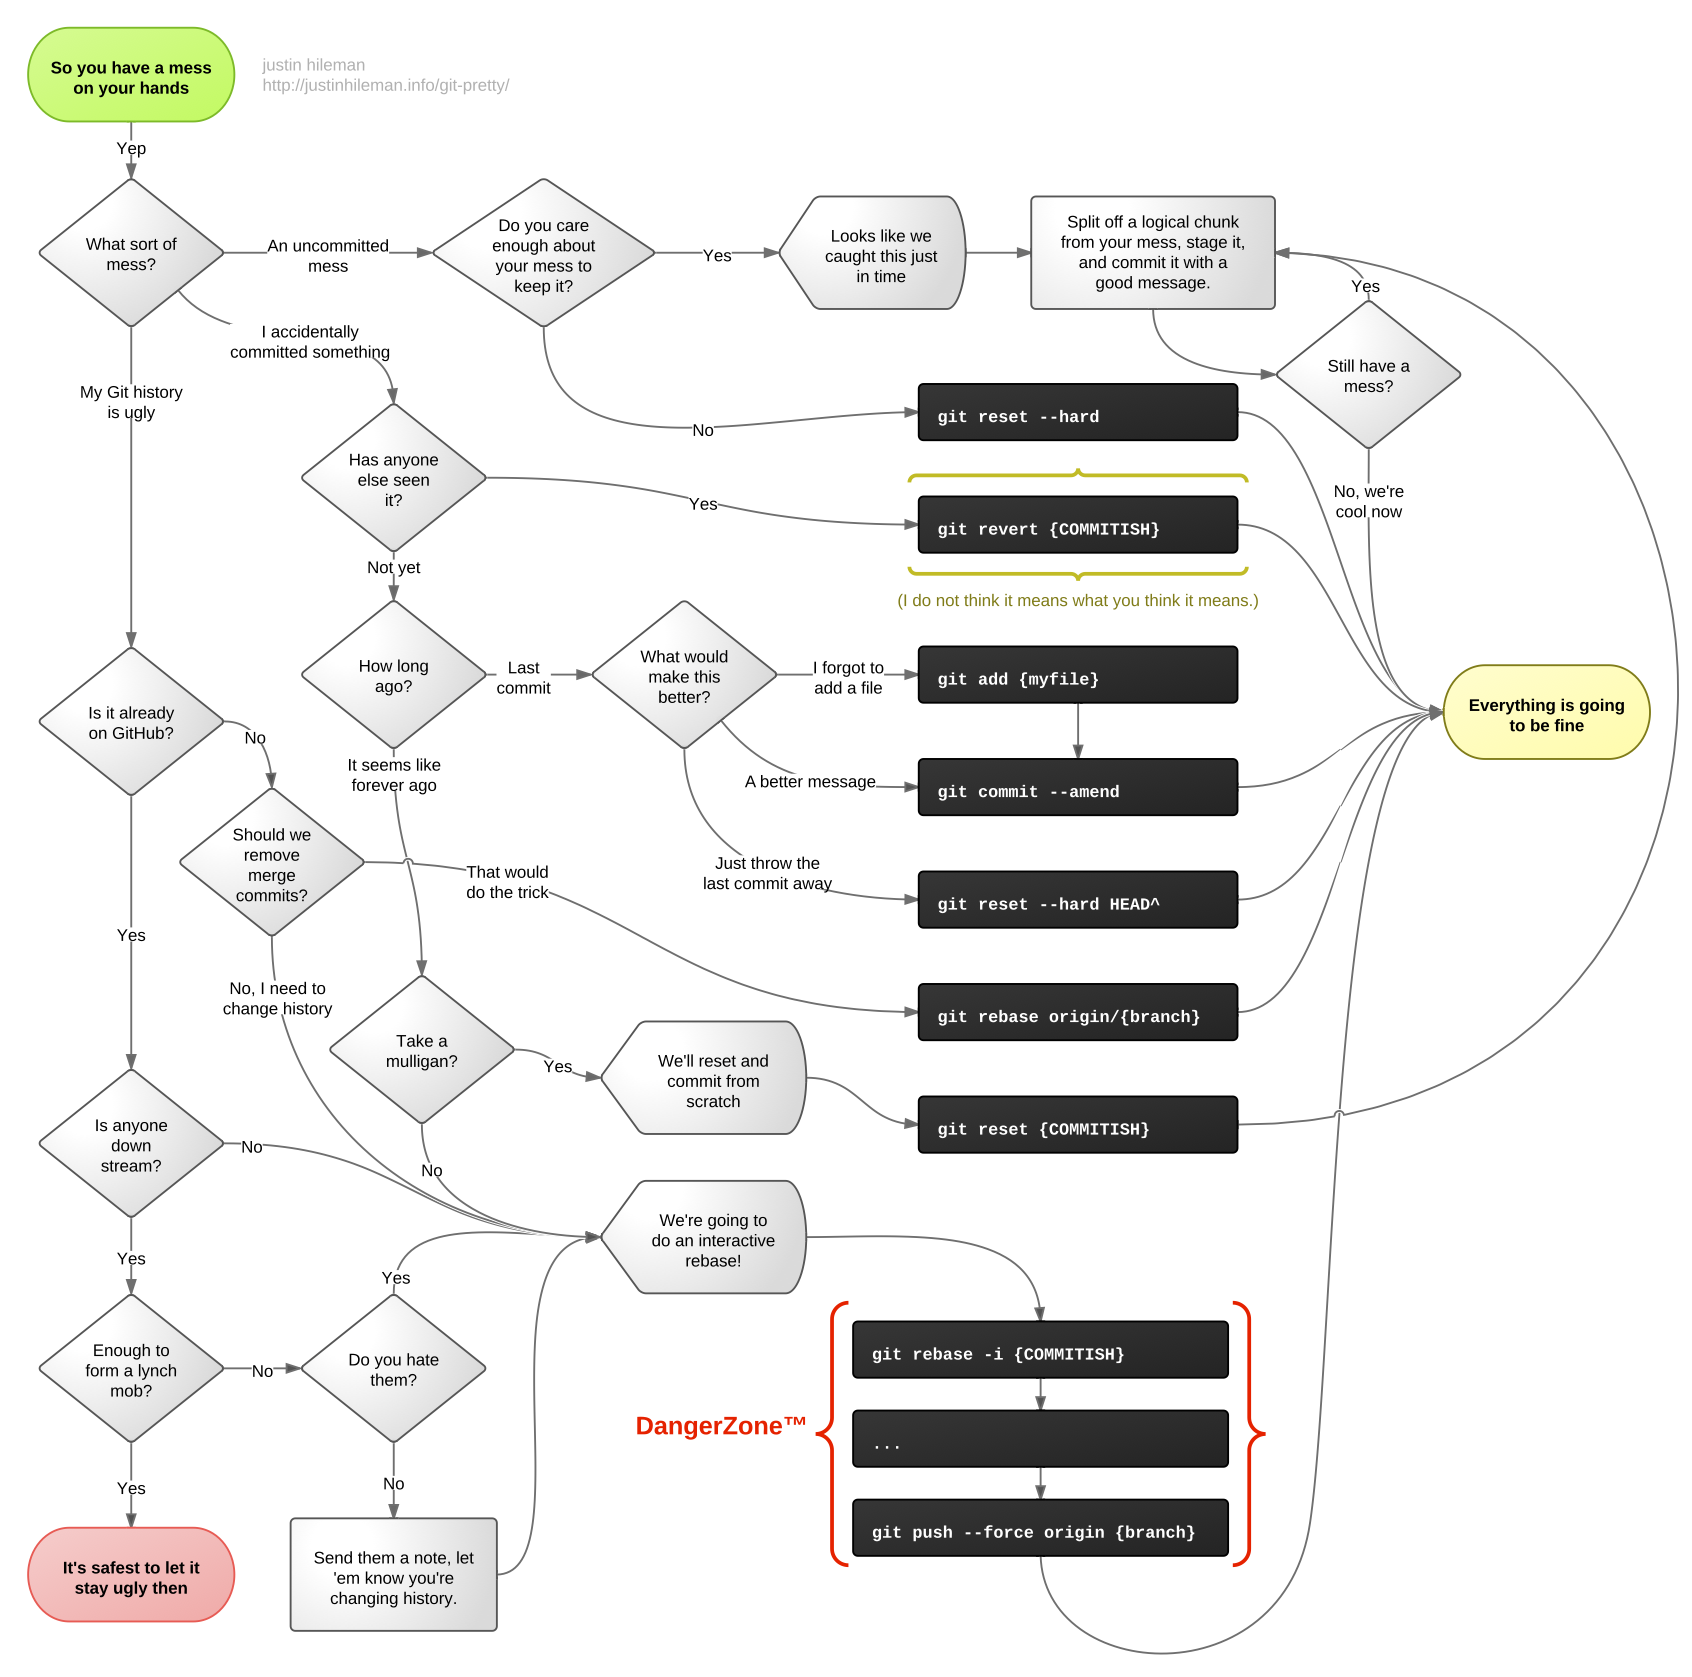
\includegraphics[scale=0.55]{img/git-pretty.png}
    	 \caption{Cambiare la storia con git}
 	\end{center}
\end{figure}

\subsection{Git Hooks}
Come molti VCS anche Git può lanciare custom scripts al verificarsi di determinate azioni. Esistono due gruppi di hooks: 
\begin{itemize}
    \item client-side: sono triggerati quando vengono eseguite operazioni come commit e merge
    \item server-side: vengono lanciati quando si eseguono operazioni sulla rete come push e pull 
\end{itemize}
\begin{center}
    \begin{tabular}{ |c|c| } 
        \hline
        \textbf{Client-side} & \textbf{Server-side} \\
        \hline
        pre-commit & pre-receive \\ 
        prepare-commit-msg & update \\ 
        commit-msg & post-receive \\ 
        post-commit & \\
        pre-rebase & \\
        post-rewrite & \\
        post-checkout & \\
        post-merge & \\
        pre-push & \\
        \hline
    \end{tabular}
\end{center}
\subsubsection{pre-commit hook}
Viene lanciato subito dopo un comando commit (prima di editare il messaggio) a meno che non si sia usata l'opzione --no-verify. Può determinare il fallimento di un commit.
\subsubsection{post-commit hook}
Viene lanciato dopo il commit (dopo che è stato accettato), quindi non ne può cambiare lo stato. Viene utilizzato solitamente per mandare delle notifiche o per \href{https://lolcommits.github.io/}{lolcommits}
\subsubsection{update (server-side)}
Possono essere utilizzati per rifiutare un push (CI con capacità di bloccare un commit) e differiscono nel come vengono chiamati.
\subsubsection{post-receive (server-side)}
Può essere usato per notificare

\subsection{Git Flow}
\noindent Fino ad ora abbiamo utilizzato i branch in maniera piuttosto "casuale". AVH ha generato un set di script (prima ad uso interno e successivamente reso pubblico) per regolamentare l'utilizzo dei branch, introducendo una tipizzazione, nuove operazioni guidate eincludendo anche i remote. Per poter cominciare ad utilizzare git flow va lanciato il comando
\begin{minted}[bgcolor=LightGray, fontsize=\footnotesize]{bash}
$ git flow init
\end{minted}
A questo punto la repo sarà gestita da git flow che si occuperà dei comandi a basso livello (git branch, git checkout) mentre a noi basterà tenere a mente le "regole" dei branch:
\begin{itemize}
    \item \textbf{master}: ramo con vita infinita che contiene le versioni stabili e pronte alla consegna
    \item \textbf{develop}: ramo con vita infinita che è considerato quello di integrazione
    \begin{figure}[H]
    	\begin{center}
        	 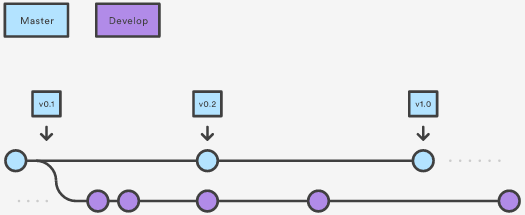
\includegraphics[scale=0.55]{img/master-develop.png}
        	 \caption{I rami master e develop non hanno fine}
        \end{center}
    \end{figure}
    \item \textbf{feature}: ramo che contiene lo sviluppo di una feature che poi andrà a confluire nel ramo develop. Non possono esserci più feature aperte con lo stesso nome
    \begin{minted}[bgcolor=LightGray, fontsize=\footnotesize]{bash}
$ git flow feature start feat1
#hack hack hack 
$ git flow feature finish feat1
    \end{minted}
    \begin{figure}[H]
    	\begin{center}
        	 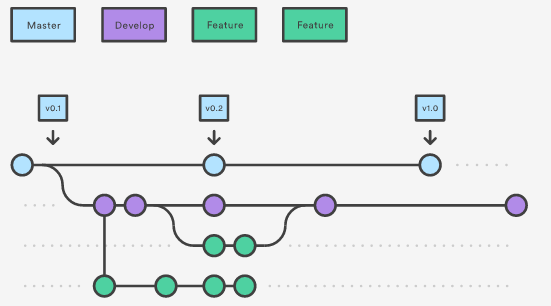
\includegraphics[scale=0.55]{img/feature.png}
        	 \caption{Il ramo feature confluisce nel ramo develop}
     	\end{center}
    \end{figure}
    
    \item \textbf{release}: è il ramo che si posiziona tra develop e produzione. Viene creata una release quando si vuole "congelare" lo stato del mio prodotto che verrà mandato in produzione.
    \begin{minted}[bgcolor=LightGray, fontsize=\footnotesize]{bash}
$ git flow release start ver1
#test fix test fix
$ git flow release finish ver1
    \end{minted}
    \begin{figure}[H]
    	\begin{center}
        	 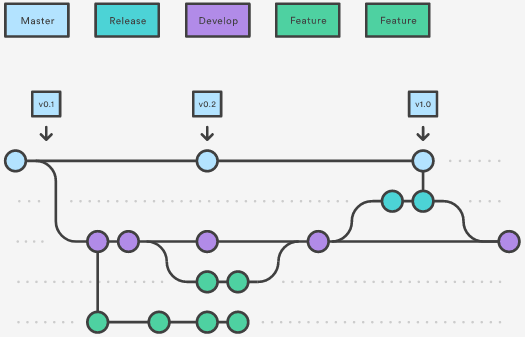
\includegraphics[scale=0.55]{img/release.png}
        	 \caption{Ramo release}
     	\end{center}
    \end{figure}
    
    \item \textbf{hotfix}: ramo dove ci sono le riparazioni veloci dei difetti urgenti che non possono aspettare una prossima release
    \begin{minted}[bgcolor=LightGray, fontsize=\footnotesize]{bash}
$ git flow hotfix start hotfix1
#hack hack hack
$ git flow hotfix finish hotfix1
    \end{minted}
    \begin{figure}[H]
    	\begin{center}
        	 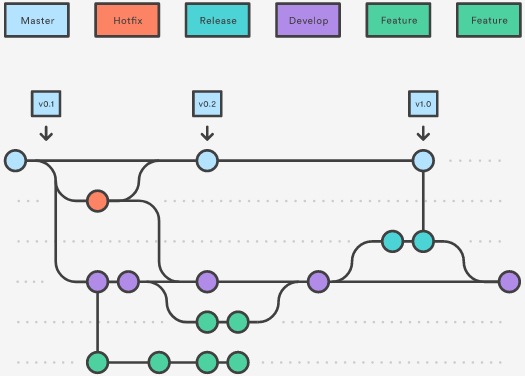
\includegraphics[scale=0.55]{img/hotfix.png}
        	 \caption{Ramo hotfix}
     	\end{center}
    \end{figure}
    \item \textbf{support}: ramo che serve per fornire supporto a versioni vecchie del sw (non è molto usato)
\end{itemize}

\subsection{Autorizzazioni e revisioni}
Possiamo accorgerci di alcuni limiti di git: abbiamo un singolo livello di autorizzazione e nessun livello di review

\begin{minted}[bgcolor=LightGray, fontsize=\footnotesize]{bash}
$ git request-pull <start> <url> [<end>]
\end{minted}
È il comando che viene utilizzato per generare un riassunto del lavoro fatto su una determinata repo, utilizzato in passato per convincere altri a pullare il codice (ti faccio vedere cosa ho fatto quindi sei più motivato a scaricare il mio codice). \\\\

\noindent La maggior parte dei progetti open source soffre di questi limiti. Gli ambienti di hosting hanno cercato di trovare soluzioni alternative inventandosi nuovi meccanismi e cercando di imporre nuovi workflow.\\

\noindent \textbf{Fork}: risolve un primo problema di autorizzazioni perchè permette di mantenere i legami tra la repository originale  e la mia forkata, ma con owner e autorizzazioni diverse. Sulla mia repo forkata ho permessi di scrittura, ma non posso scrivere sulla repo originale. I file che non vengono modificati (ossia di cui non cambia il blob) non vengono duplicati, ma viene mantenuto un puntatore alla repo originale.\\
Tra creazione e deploy è prevista una fase di review: rimane il controllo della repo originale. Ho forkato una repo, ho fatto un bug fix, mando una pull (merge) request, dove viene revisionato il mio codice.\\
\begin{figure}[H]
	\begin{center}
    	 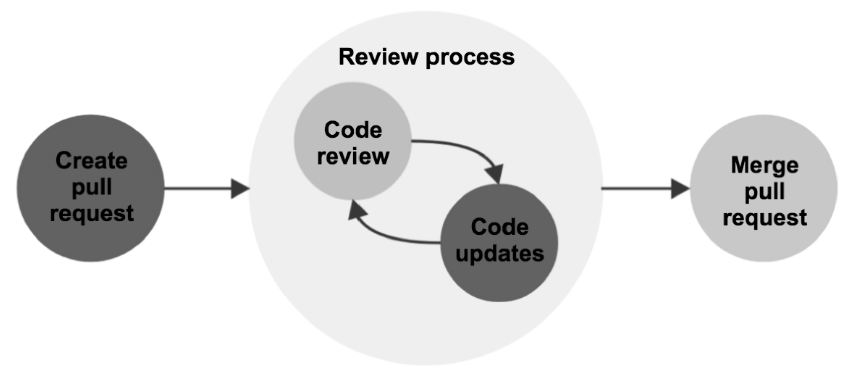
\includegraphics[width=\linewidth]{img/deployreview.png}
    	 \caption{Processo di revisione di una pull/merge request}
 	\end{center}
\end{figure}
\noindent\textbf{Pull/merge request}: permette di gestire interazioni lasche tra sviluppatori mediate dal sito di hosting.
Per creare una pull/merge request sono necessari:
\begin{itemize}
    \item titolo della pull request
    \item target branch
    \item source branch
\end{itemize}
Sotto la richiesta si genera un thread di discussione tra sviluppatori che possono fare da garanti o discutere sulla pull/merge request.

\subsubsection{Gerrit}
È un progetto di google AOSP: l'obiettivo è quello di rendere decentralizzata anche la fase di review tramite delle peer review di sottomissioni. \\
Ci sono due ruoli principali:
\begin{itemize}
    \item Verifier: scarica il codice da verificare sulla propria macchina, esegue la build e i test e comunica allo sviluppatore il risultato aggiungendo un messaggio di spiegazione
    \item Approver: deve verificare che la modifica proposta passi in maniera positiva un set di domande e poi la può marcare come LGTM (Looks Good To Me)
\end{itemize}
La sua architettura è abbastanza semplice e può essere pensata come due git server:
facciamo un push su un git server (dove hanno accesso in lettura i reviewer e dove gli altri possono solo scrivere), i reviewer approvano e "spostano" sul git server pubblico, che tutti possono vedere e leggere.\\
L'hash non è più del file ma del changeset, quindi si fa un versionamento della modifica.


\begin{figure}[H]
	\begin{center}
    	 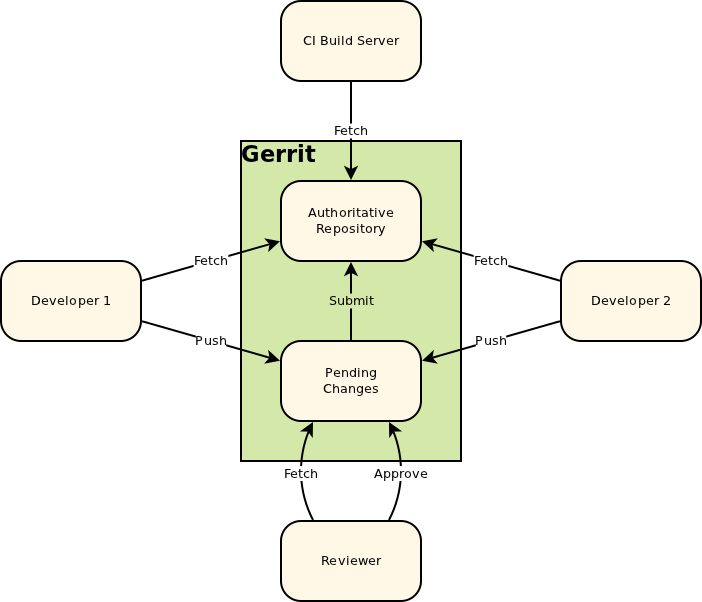
\includegraphics[scale=0.4]{img/gerrit.png}
    	 \caption{Processo di revisione di una pull/merge request}
 	\end{center}
\end{figure}

